\chapter{Library structure}

	To make it a bit easier to work with the library, I will give an overview
	of its structure. This way, you'll have a general idea about how the
	library works.
	
	\section{The VoIP session}
	
	The central concept in the library is that of a VoIP session. To add VoIP
	to an application, you first create a session with the desired parameters
	(like the sampling rate). You can then add destinations to the session,
	join multicast groups, etc. When you no longer need VoIP, you simply have
	to destroy the VoIP session.
	
		\subsection{Creating a session}
		
		More specific, a VoIP session is represented by the {\tt JVOIPSession} class.
		You create a session by calling the {\tt Create} function, which takes a
		parameter of type {\tt JVOIPSessionParams}. As the name suggests, this class
		contains the parameters for the session.
		
		The {\tt JVOIPSessionParams} class takes parameters for the sample interval, the
		input sampling rate, the output sampling rate, compression type, etc. It
		also contains parameters for each component (for example the RTP
		transmission module). These parameters are stored in classes derived from
		{\tt JVOIPComponentParams}.
		
		For example, if you specified in a {\tt JVOIPSessionParams} instance that you
		want to use the RTP transmission module, you can specify parameters --
		like the portbase -- for this module by passing an instance of
		{\tt JVOIPRTP\-Trans\-mis\-sion\-Params} to {\tt JVOIPSessionParams}. You can do this by using
		the {\tt JVOIPSessionParams} member function {\tt Set\-Trans\-mis\-sion\-Params}.
		
		All this is represented in the UML diagram in figure \ref{create-session-schema}.
		\begin{figure}
			\center
			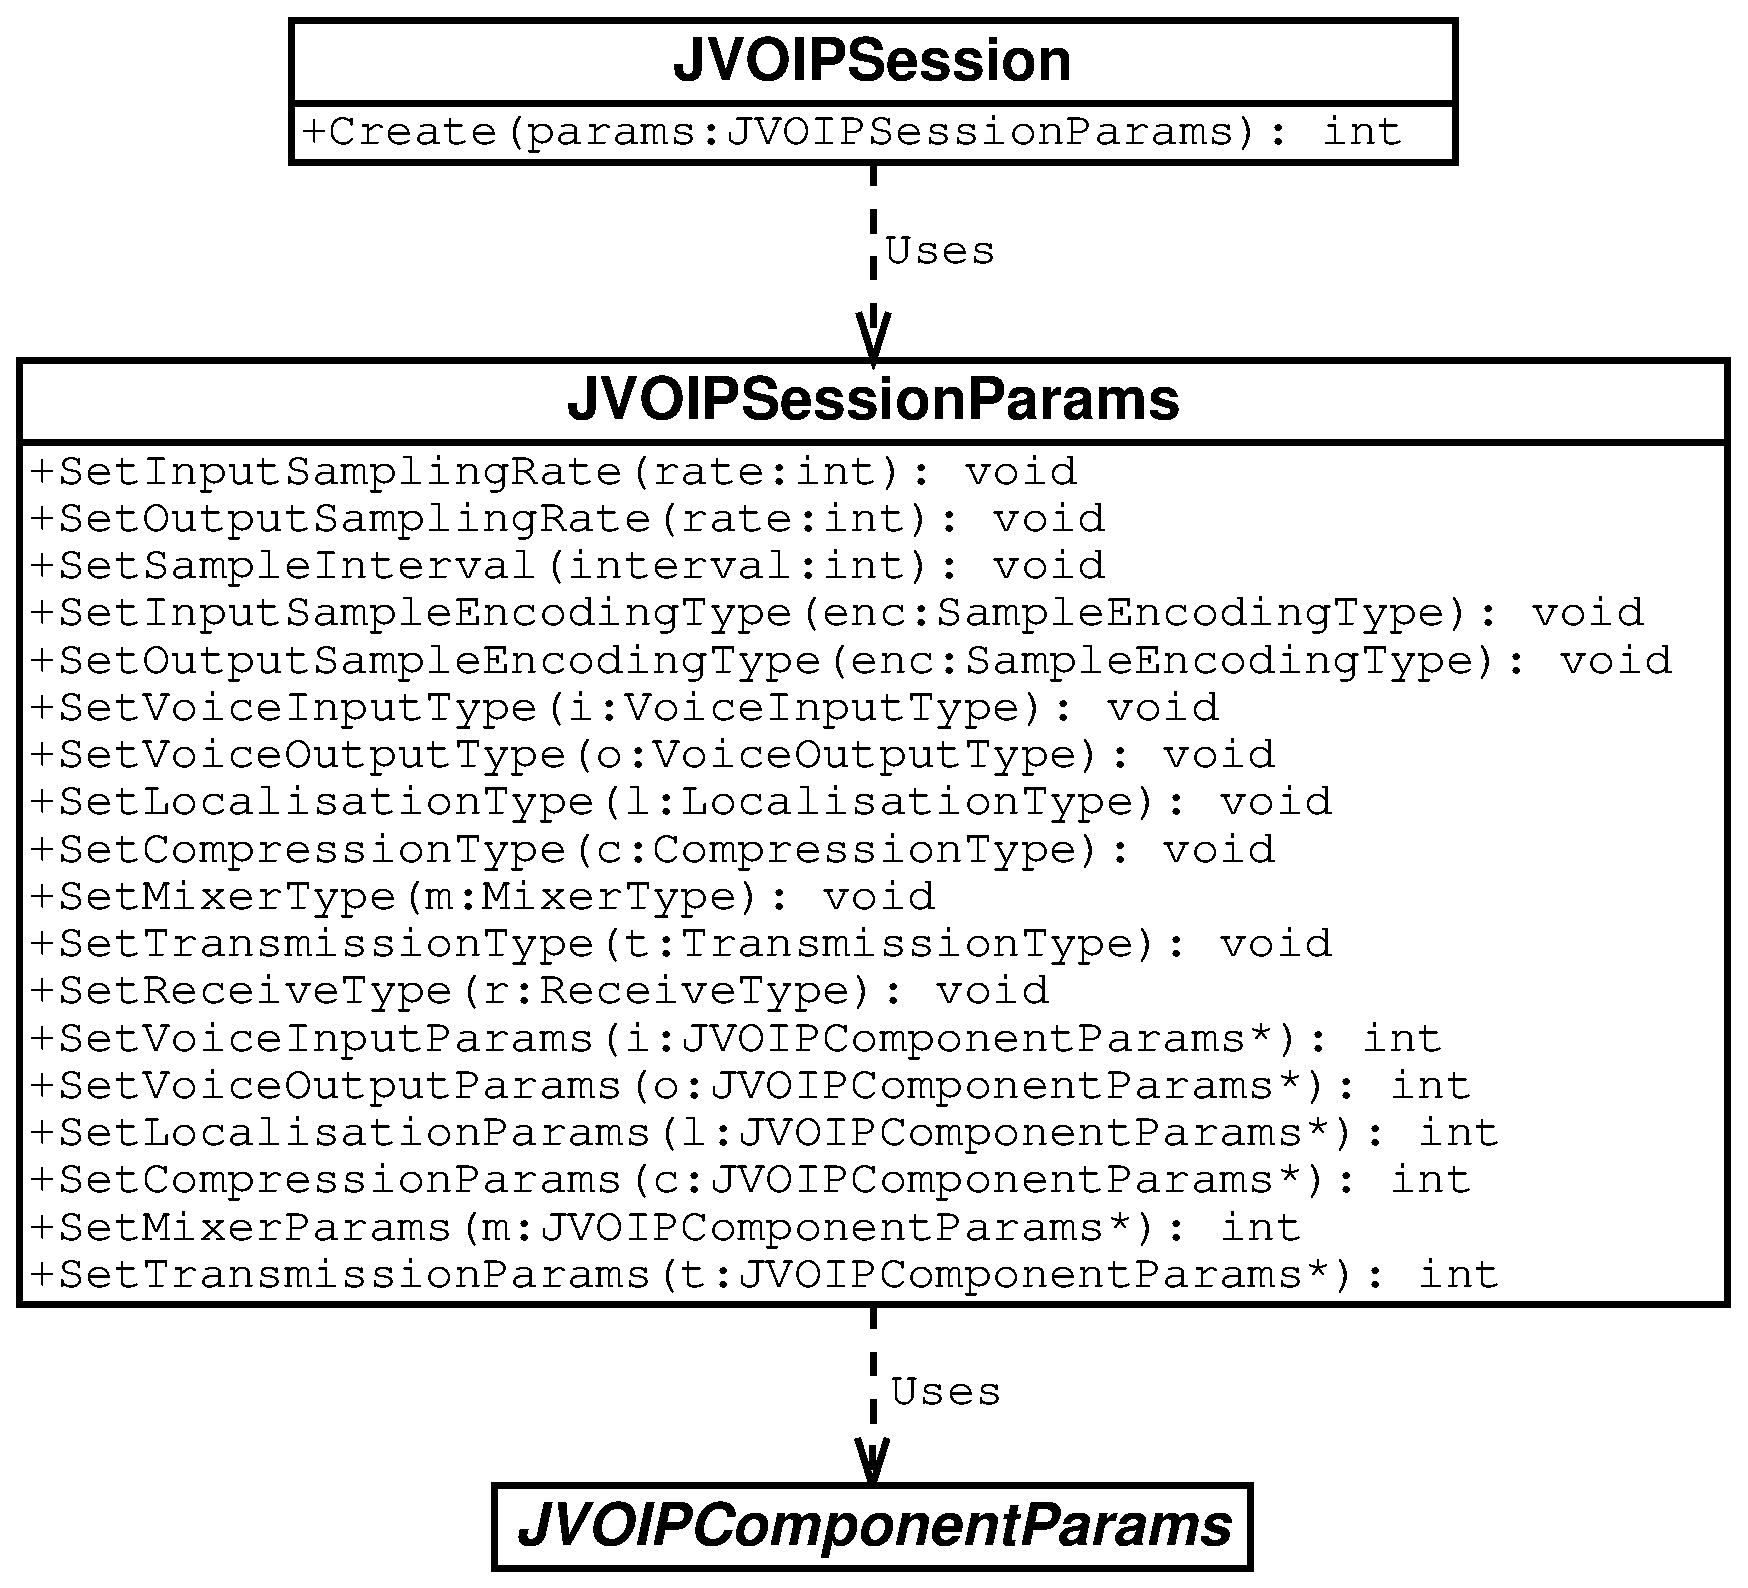
\includegraphics[width=0.85\linewidth]{images/manual/chapter2/create-session-schema.eps}
			\caption{Creating a session}
			\label{create-session-schema}
		\end{figure}
		
		\subsection{An active session}
		
		Once the session is active, you can still change several attributes. The
		functions to do this are similar to the functions used in
		{\tt JVOIPSessionParams}. These operations are represented in the UML diagram in
		figure \ref{change-session-params}
		\begin{figure}
			\center
			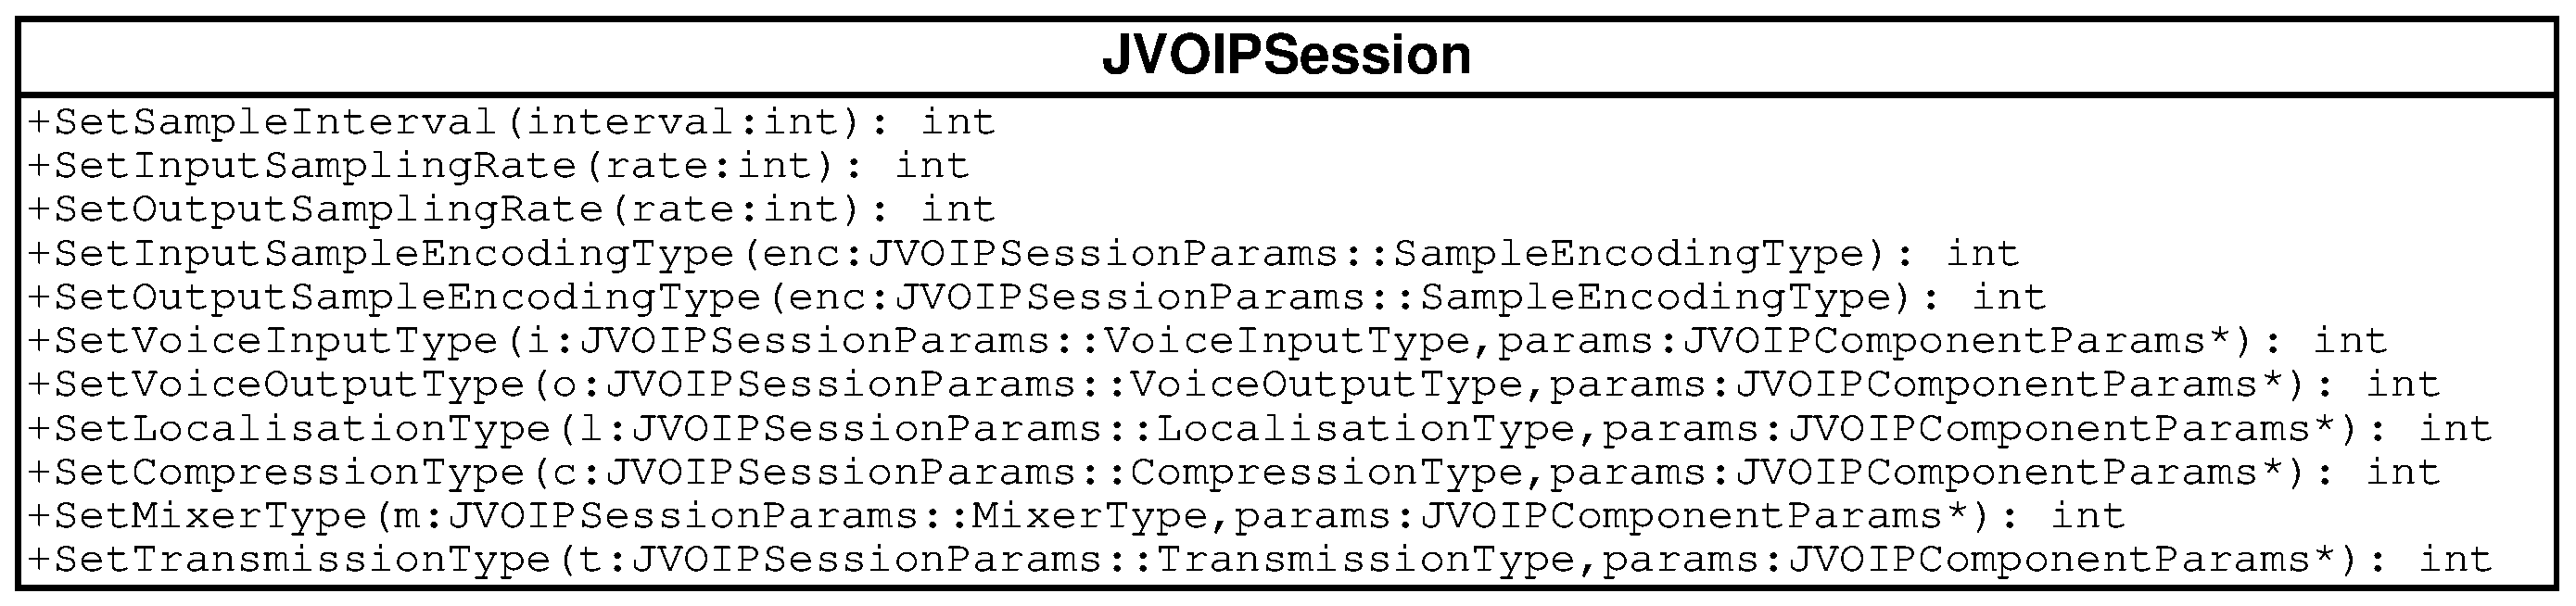
\includegraphics[width=\linewidth]{images/manual/chapter2/change-session-params.eps}
			\caption{Changing attributes of an active session}
			\label{change-session-params}
		\end{figure}
		
		Now that you have a working session, you still have to specify where the
		VoIP data has to be sent to. With the {\tt JVOIP\-Ses\-sion} member functions
		{\tt Add\-Destina\-tion} and {\tt Delete\-Destina\-tion}, you can specify
		both unicast and multicast destinations. To be able to receive data which is sent
		to a specific multicast group, you must first join that group. Joining and leaving
		multicast groups can be done by using the functions {\tt JoinMulticastGroup} and
		{\tt LeaveMulticastGroup}.
		
		You can also specify which incoming data you are willing to accept. You
		can accept all incoming data, you can specify the IP-port combinations
		which should be ignored or you can specify the IP-port combinations which
		should be accepted. In the latter case, all packets coming from other
		sources are discarded.
		
		The functions that determine where VoIP data is sent and what VoIP data
		is accepted are depicted in figure \ref{send-and-receive-functions}.
		\begin{figure}
			\center
			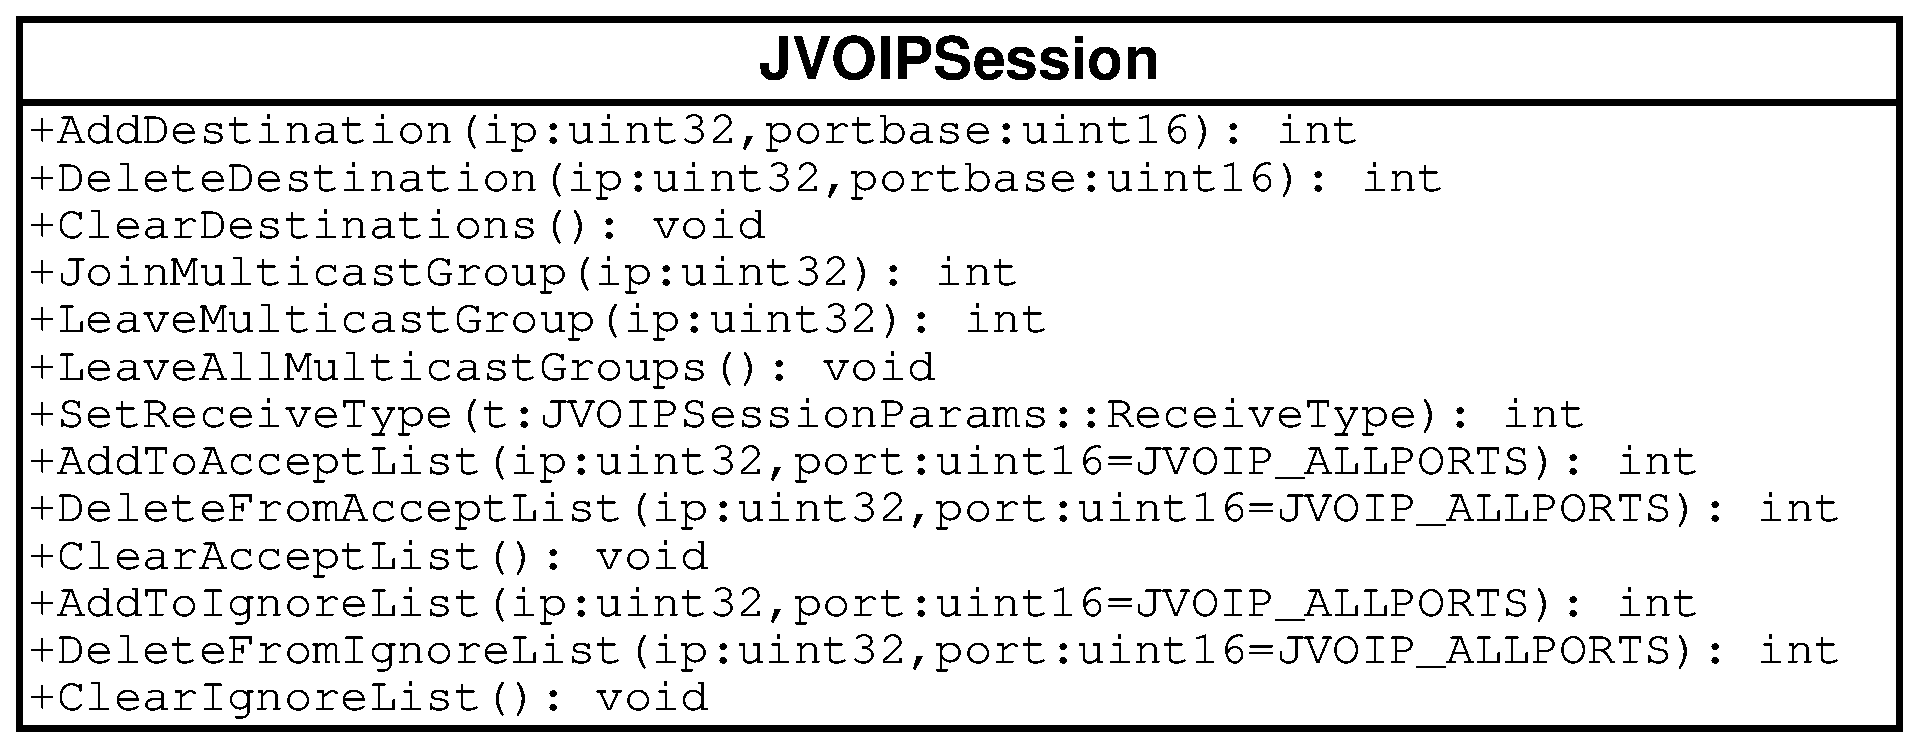
\includegraphics[width=0.9\linewidth]{images/manual/chapter2/send-and-receive-functions.eps}
			\caption{Functions for sending and receiving}
			\label{send-and-receive-functions}
		\end{figure}
		
		\subsection{Destroying a session}
		
		Destroying a session is easy: you simply have to call the {\tt JVOIPSession}
		member function {\tt Destroy}. 

		{\bf IMPORTANT! }
		{\it As of version 1.2.0 it is no longer allowed to rely on the session's destructor
		to destroy the session. This is so because it can cause problems when a class is
		inherited from {\tt JVOIPSession}. See appendix A for a
		detailed explanation.}
		
		\subsection{Working with user defined components}
		
		In the introduction I said that the library had functionality to use your
		own user defined components. To be able to use your own component, you
		must first register it with the library. To do this, you must inherit
		your own class from {\tt JVOIPSession} and override one of the
		{\tt RegisterUserDefinedX} functions, where the X depends on the component
		type. For example, if you would like to try your own transmission scheme,
		you would have to override the function called
		{\tt RegisterUserDefinedTransmission}. This function has an argument in which
		you can fill in a pointer to your component.
		
		Similarly, you can also override functions called
		{\tt UnregisterUserDefinedX}. These functions can come in handy when you used
		dynamically allocated memory in the registration of your component. In the
		`unregistration' functions, you can then free this memory.
		
		You'll find an overview of these functions in figure \ref{register-userdef-functions}
		\begin{figure}
			\center
			\includegraphics[width=\linewidth]{images/manual/chapter2/register-userdef-functions.eps}
			\caption{Function for registering user defined components}
			\label{register-userdef-functions}
		\end{figure}
		
		\subsection{Overridables}\label{subsection-overridables}
		
		Besides the registration functions for user defined components, there are
		also a number of other functions which are overridable. To begin with,
		there are two functions called {\tt UserDefinedCreate} and
		{\tt UserDefinedDestroy} The first one is called when the VoIP session is
		about to start (it is called from the {\tt Create} function). The second one
		is called when the session is about to end. These functions can be called
		when you need to perform specific actions at these points.
		
		There is also a function available to perform an action after each
		sampling interval. This function is called {\tt IntervalAction}. You'll find
		more information about this function later on.
		
		It is always possible that the VoIP thread ends due to some external
		circumstances. To be able to detect this, there is a function called
		{\tt Thread\-Fi\-nished\-Handler} which will be called whenever the VoIP session
		thread ends. Its parameters will contain information about what caused
		the thread to end.
		
		Finally, there are also overridable functions for the 3D localisation support.
		To be able to add 3D effects to the sound, you must override three functions:
		{\tt RetrieveOwnPosition}, {\tt EncodeOwnPosition} and {\tt Decode\-Positional\-Info}.
		
		An overview of these overridable functions is given in figure \ref{overridable-functions}
		\begin{figure}
			\center
			\includegraphics[width=\linewidth]{images/manual/chapter2/overridable-functions.eps}
			\caption{Other overridable functions}
			\label{overridable-functions}
		\end{figure}
		
	\section{The VoIP framework}\label{text-voipframework}
	
	The library uses a VoIP framework to define how components should work together.
	In this section we'll take a closer look at how all this works. The classes of the
	VoIP framework are all in the namespace {\tt VoIPFramework}.
	
		\subsection{A voice information container}
		
		The central data structure in the VoIP framework is the {\tt VoiceBlock} class.
		This class provides the functionality to store the voice data, the localisation
		data and information about sampling rate, compression, etc.
		
		\subsection{The framework base classes}
		
		The VoIP framework defines several base classes which represent different
		components needed for a VoIP call:
		
		\begin{itemize}
		\item {\tt SamplingTimer}\\
			Determines when a sample interval has elapsed.
		
		\item {\tt SampleInput}\\
			This class provides the voice data that needs to be transmitted.
		
		\item {\tt SampleOutput}\\
			Represents some kind of output device for the samples to be sent
			to.
		
		\item {\tt Location3D}\\
			A component which can add 3D information to the voice block. This
			information can then be used by {\tt Transform3D} to add a 3D
			effect to the voice data.
		
		\item {\tt Transform3D}\\
			Uses the information provided by a {\tt Location3D} component
			to add a 3D effect to the sound.
		
		\item {\tt VoiceCompressor}\\
			Compresses the voice data.
		
		\item {\tt VoiceDecompressor}\\
			Decompresses the voice data.
		
		\item {\tt VoiceMixer}\\
			Makes sure that samples are delivered to the {\tt SampleOutput}
			component at the correct time. Should also mix several voice
			streams together.
		
		\item {\tt VoiceTransmitter}\\
			Transmits and receives the information contained in a {\tt VoiceBlock}
			instance.
		\end{itemize}
		
		\subsection{The VoIP procedure}\label{text-voipframework-voipprocedure}
		
		The class {\tt VoiceCall} is what actually makes VoIP possible. Besides some
		initialization functions, it contains a member function called {\tt Step}. Each
		time that function is called, it checks if a sample interval has passed and if
		so, it processes the data from that interval. The {\tt Step} routine is displayed
		in pseudocode in figure \ref{voip-step-procedure}.
		
		\begin{figure}
			\begin{tabular}{|p{1.1\linewidth}|}
				\hline
				\begin{minipage}{0.95\linewidth}
				\begin{lstlisting}{}
Step()
{
	if (samplingtimer->HasTimeOut())
	{
		sampleinput->GetSampleBlock(&block);
		sampleinput->StartSampling();
		voicemixer->GetSampleBlock(&block2);
		sampleoutput->Play(&block2);
		samplingtimer->RestartTimer();

		if (location3d != NULL)
			location3d->Add3DInfo(&block);
		if (voicecompressor != NULL)
			voicecompressor->Compress(&block);
		voicetransmitter->SendBlock(&block);

		voicemixer->GetSampleOffset(&sampleoffset);
		voicetransmitter->SetSampleOffset(sampleoffset);

		voicetransmitter->Poll();
		voicetransmitter->StartVoiceSourceIteration();
		for (each voice source with available data)
		{
			sourceid = voicetransmitter->GetVoiceSourceID();
			do
			{
				voicetransmitter->GetSampleBlock(&block);
				if (voicedecompressor != NULL)
					voicedecompressor->Decompress(&block,sourceid);
				if (transform3d != NULL)
					transform3d->Create3DEffect(&block,sourceid);
				voicemixer->AddBlock(&block,sourceid);
			} while (voice source has more data);
		}
		voicetransmitter->EndVoiceSourceIteration();
	}
	return 0;
}
				\end{lstlisting}
				\end{minipage}\\
				\hline
			\end{tabular}
			\caption{The {\tt Step} procedure}
			\label{voip-step-procedure}
		\end{figure}
		
		Now lets examine this routine. First of all, there is some work that
		needs to be done right away to preserve consistency in the input and
		output signals. When a sample interval has passed, we need to retrieve
		the samples from that interval and and start sampling again. We also
		need to get new data for playback and send this data to the output module.
		Finally, we have to make sure that the timer is running again. All this
		is done in the following piece of code:
		\begin{lstlisting}[frame=tb]{}
		sampleinput->GetSampleBlock(&block);
		sampleinput->StartSampling();
		voicemixer->GetSampleBlock(&block2);
		sampleoutput->Play(&block2);
		samplingtimer->RestartTimer();
		\end{lstlisting}
		
		The block with samples that we captured from the input device can then
		be processed futher. If 3D effects are required, we can add 3D information
		(e.g. the current position in the 3D environment) to the block. If
		compression is desired, the block is then passed through a compression
		routine. Afterwards, the block can be passed on to the transmission module
		which can send it to the required destinations. The code below is responsible
		for doing all this.
		\begin{lstlisting}[frame=tb]{}
		if (location3d != NULL)
			location3d->Add3DInfo(&block);
		if (voicecompressor != NULL)
			voicecompressor->Compress(&block);
		voicetransmitter->SendBlock(&block);
		\end{lstlisting}
		
		Each {\tt VoiceBlock} instance delivered to the mixer will have a specific
		sample offset. This sample offset determines when the samples in the block
		should be played back. Now, the mixer keeps track of the sample offset of the
		first sample in its buffers. Obviously, this offset changes whenever the mixer
		passes data on to a {\tt SampleOutput} component.
		
		In the next piece of code, the {\tt Step} routine asks the mixer for this
		sample offset and it gives this value to the transmitter.
		\begin{lstlisting}[frame=tb]{}
		voicemixer->GetSampleOffset(&sampleoffset);
		voicetransmitter->SetSampleOffset(sampleoffset);
		\end{lstlisting}
		
		Now why is this necessary? Well, each incoming data stream will have sample
		offset information relative to that stream, but this has nothing to do with
		at what local sample offset each sample should be played back. Using the
		current sample offset information we can create a mapping between remote
		and local offsets when a new stream of data is coming in.
		
		In the last chunk of code, we'll process the incoming voice data. First,
		the transmission module is instructed to poll for new data. When this
		is done, we'll iterate over the sources which have new data available
		and we will process each source's data.
		\begin{lstlisting}[frame=tb]{}
		voicetransmitter->Poll();
		voicetransmitter->StartVoiceSourceIteration();
		for (each voice source with available data)
		{
			sourceid = voicetransmitter->GetVoiceSourceID();
			do
			{
				voicetransmitter->GetSampleBlock(&block);
				if (voicedecompressor != NULL)
					voicedecompressor->Decompress(&block,sourceid);
				if (transform3d != NULL)
					transform3d->Create3DEffect(&block,sourceid);
				voicemixer->AddBlock(&block,sourceid);
			} while (voice source has more data);
		}
		voicetransmitter->EndVoiceSourceIteration();
		\end{lstlisting}
		
		As you can see, the actual iteration is between a call to {\tt Start\-Voice\-Source\-Iteration}
		and {\tt End\-Voice\-Source\-Iteration}. These functions can be useful
		when you're working with multiple threads. To avoid that things get nasty,
		you could use the former functions to lock and unlock a mutex that
		controls the access over the transmission component (this is the way I use
		these functions).
		
		Inside the iteration you can see that for each voice source, all sample blocks
		are retrieved, decompressed and that 3D effects are added to the sound if
		necessary. Then, the samples are passed on to the mixer which can insert them
		at the right position inside its buffers.
		
		The transmission module should provide a unique identifier for each source of
		voice data. The compression module and the 3D effect module can use this
		value to identify stored information about a specific source.
		
	\section{The components}
	
	Now that you have a basic idea of what the session can do, we can examine
	the components themselves and how they interact with each other and with the
	session.
	
		\subsection{Base component class}
		
		All components (transmission, input, \ldots) are derived from the class
		{\tt JVOIP\-Com\-po\-nent}, which is illustrated in figure \ref{base-component-class}.
		The {\tt JVOIP\-Com\-po\-nent} base class defines some functions which each
		component {\em must} implement.
		\begin{figure}
			\center
			\includegraphics[width=0.85\linewidth]{images/manual/chapter2/base-component-class.eps}
			\caption{The base component class}
			\label{base-component-class}
		\end{figure}
		
		First of all, there are the {\tt GetComponentState} and {\tt SetComponentState}
		functions. Why are these functions necessary? Well, suppose you have an input
		module that reads sound data from a file and at some point, you would like to switch
		to soundcard input.
		
		The VoIP session then first de-initializes the current input
		routine. It is necessary that the current component is first de-initialized because
		it may have exclusive access to a resource that the new module also wishes to use.
		If the resource isn't freed first, the new component can't be initialized.
		
		The session should then initialize the new module, the soundcard input module in
		our example. But suppose that something goes wrong and the initialization fails.
		The best solution is to keep going with the previous component, so we have to
		re-initialize the file input component.
		
		At this point however, there will be inconsistency in the voice data that we're
		sending: since we have just initialized the file input module, it will start
		sending data from the beginning of the file, and not from the point where we
		left off. The solution is to save the state of the old component before it is
		de-initialized and to restore that state when the component is initialized
		again.
		
		The {\tt GetComponentState} fills in a component's current state in an instance
		of a class derived from {\tt JVOIPComponentState}. The {\tt Set\-Com\-po\-nent\-State}
		member function can then use that information to restore a component's state.
		
		The other functions are used to provide an easy way to retrieve information
		about a component. You can ask a component for its name, for a description of
		itself or you can ask its parameters. These parameters were passed to it
		during its initialization as an instance of a class derived from
		{\tt JVOIP\-Component\-Params}. The parameters can be retrieved as a vector
		where each element describes a parameter by its name and its value. Both name
		and value are stored as strings.
		
		\subsection{Component types}
		
		The VoIP framework already identified some base classes and their functions to make
		a VoIP call possible. We will now define components with some extra functionality
		which is useful for the library. Most of these components inherit from one or
		more of the framework base classes.
		
			\subsubsection{JVOIPVoiceInput}
			
			The class {\tt JVOIPVoiceInput} is shown in figure \ref{class-jvoipvoiceinput}. As
			you can see, this class inherits from {\tt SampleInput} in the {\tt VoIPFramework}
			namespace, which means that an instance of {\tt JVOIPVoiceInput} can be used in
			the {\tt Step} function, explained in \ref{text-voipframework-voipprocedure}.
			\begin{figure}
				\center
				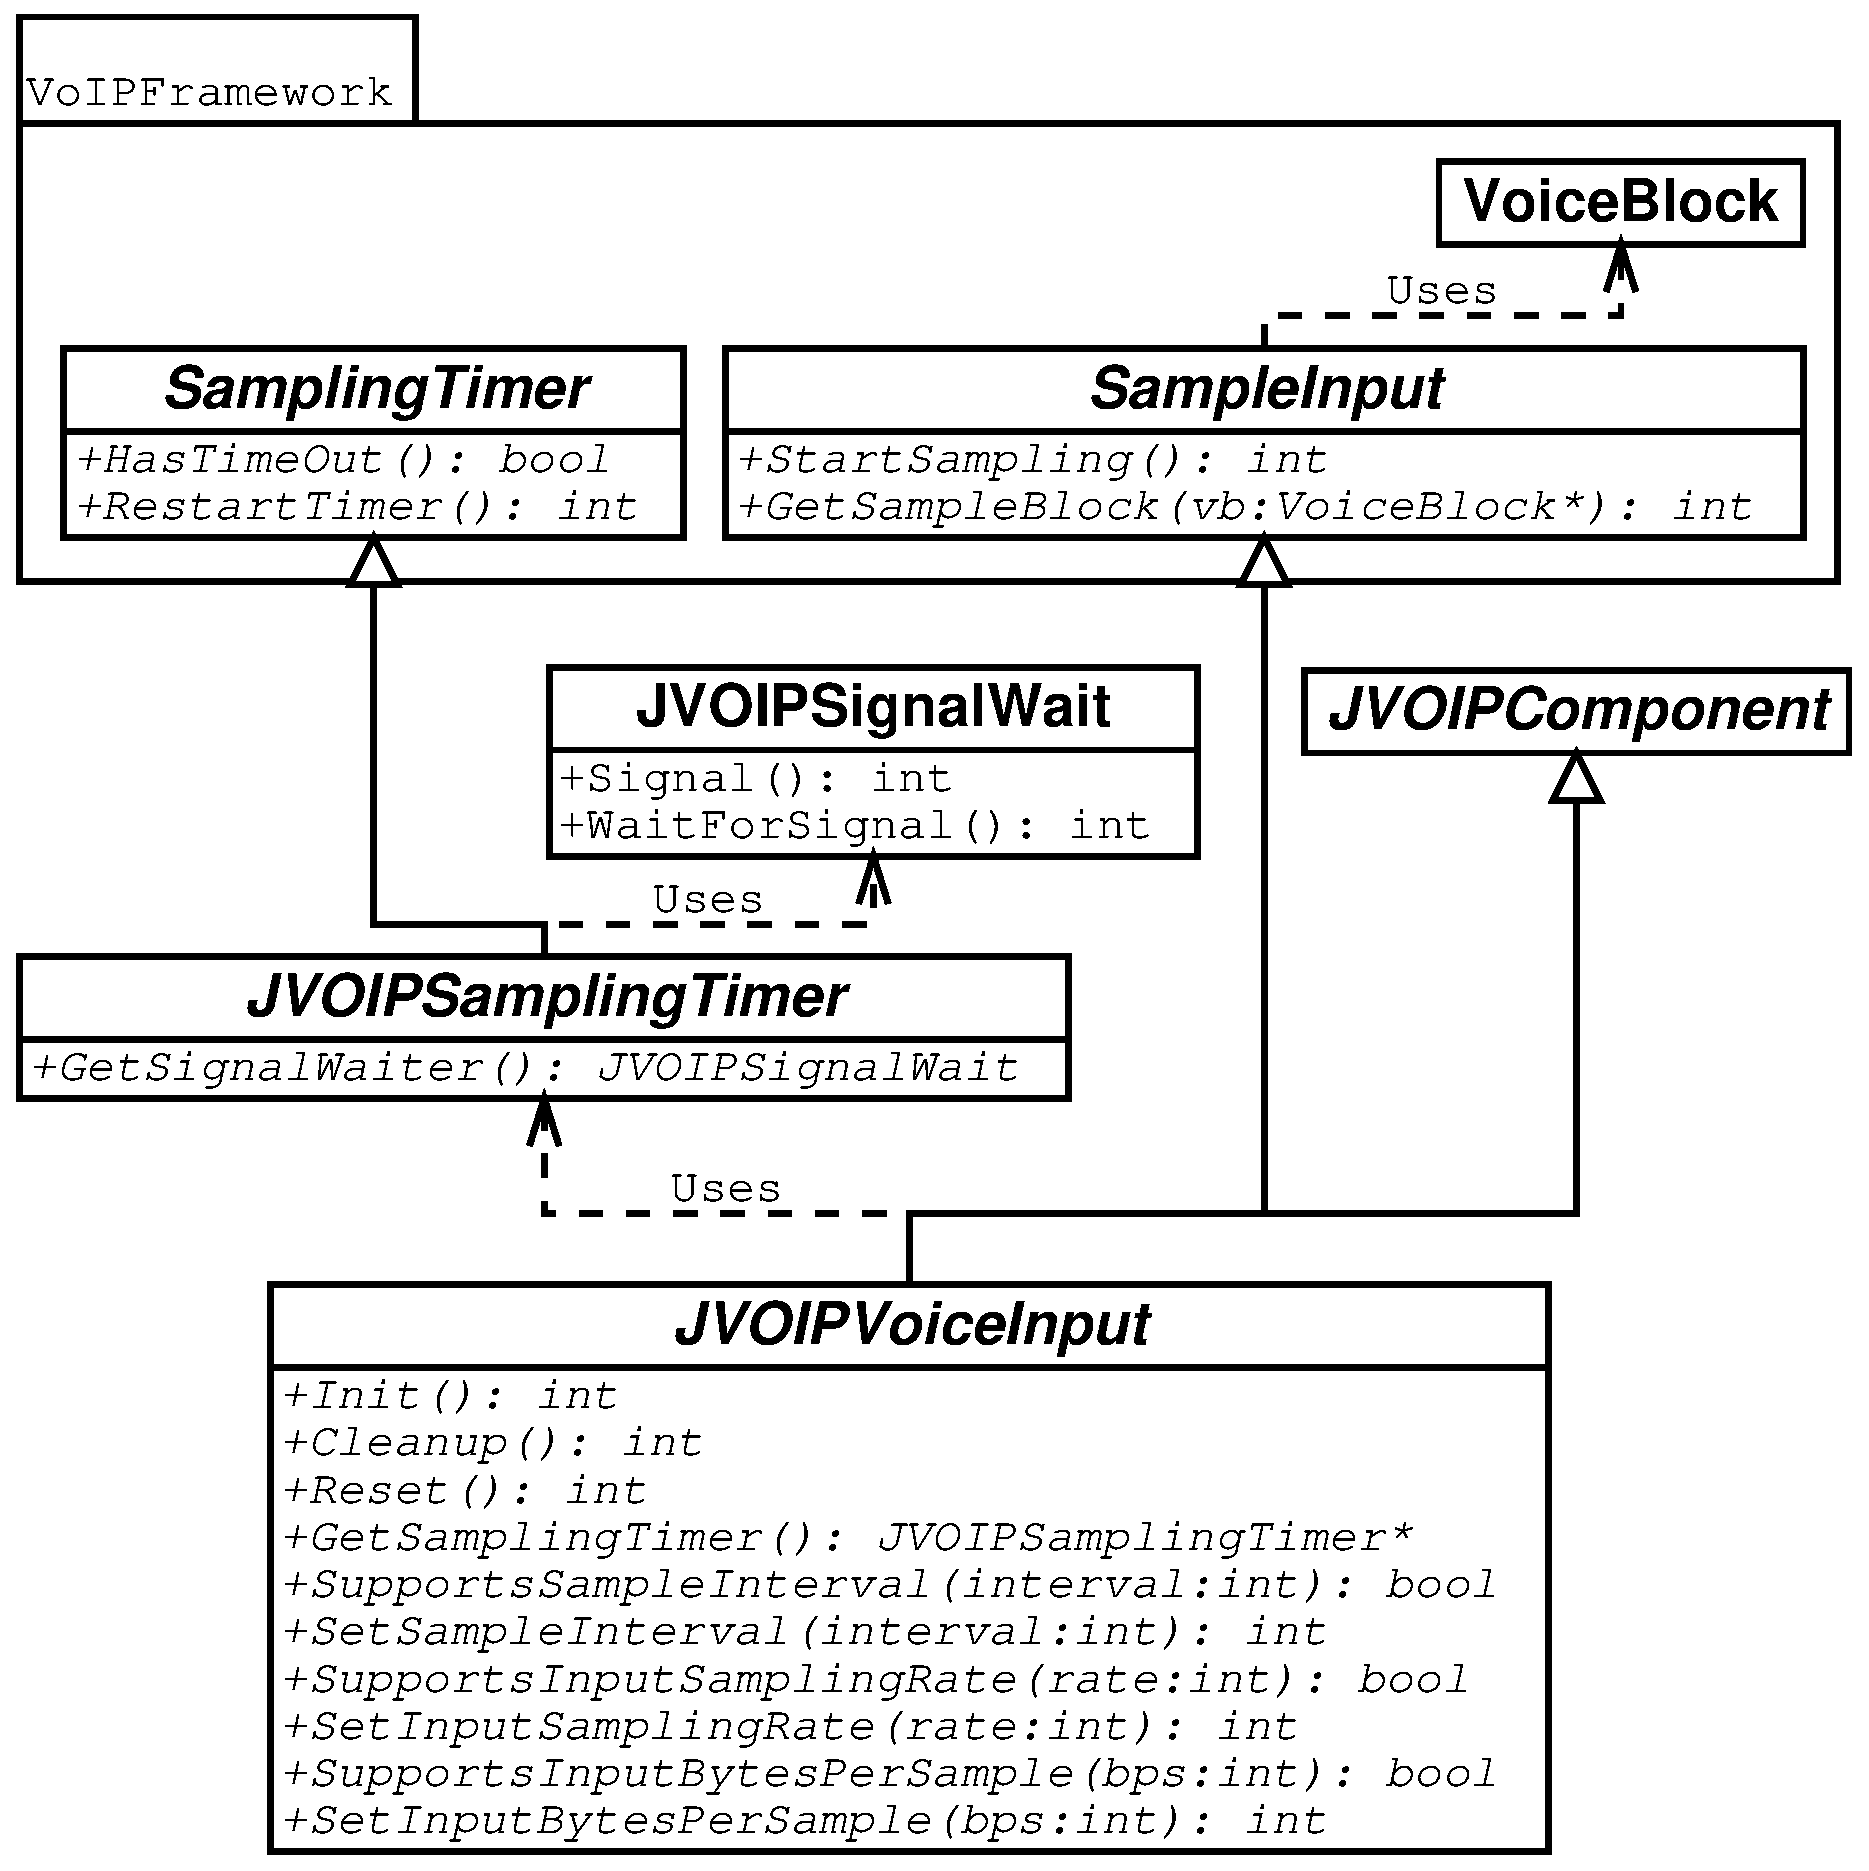
\includegraphics[width=0.9\linewidth]{images/manual/chapter2/class-jvoipvoiceinput.eps}
				\caption{JVOIPVoiceInput}
				\label{class-jvoipvoiceinput}
			\end{figure}
			
			The {\tt Init} member function of {\tt JVOIPVoiceInput} does have some parameters
			(displaying them in the figure would make the image too large). The actual syntax
			of the {\tt Init} function is this:
			\begin{center}
				{\tt
				\begin{tabular}{rl}
					int Init (&int sampinterval, int inputsamprate, \\
					&int inputbytespersample,\\
					&const JVOIPComponentParams *componentparams )\\
				\end{tabular}
				}
			\end{center}
			The VoIP session initializes the input module with the requested sample interval,
			the sampling rate and the number of input bytes per sample. It also passes the
			component specific parameters.
			
			The sampling rate and bytes per sample parameters need to be passed to the
			input module because the data it fills in in a {\tt VoiceBlock} instance should
			have those characteristics. The sample interval parameter needs to be passed
			for two reason. First, it can be useful for the module to know the interval for
			buffer allocation purposes.
			
			The second reason however, is the most important one. As is shown in figure
			\ref{class-jvoipvoiceinput}, a {\tt JVOIPVoiceInput} module has a function
			called {\tt GetSamplingTimer}. This function has to return an instance of a
			class derived from {\tt JVOIPSampling\-Timer}, which in turn is derived from
			{\tt SamplingTimer} in the {\tt VoIPFramework} namespace. As was explained
			in \ref{text-voipframework}, a class derived from {\tt SamplingTimer}
			determines when a sample interval has passed.
			
			So, since an instance of the {\tt JVOIPVoiceInput} class will deliver and
			control the timing component, it is very important that it is informed about
			the sample interval.
			
			If we take a closer look at the {\tt JVOIPSamplingTimer} component, we can see
			that this class only needs one function to be defined: {\tt GetSignalWaiter}.
			This function should return an instance of {\tt JVOIPSignalWait} which is
			controlled by the timer.
			
			To explain the use of the signal waiter, recall the {\tt Step function} of
			section \ref{text-voipframework-voipprocedure}. Since this function checks
			whether a sample interval has passed or not, you could make a VoIP call possible
			by doing something like this:
			\begin{lstlisting}[frame=tb]{}
while(true)
{
	voicecall.Step();
}
			\end{lstlisting}
			This would work very well, but there is one major disadvantage: because of the
			tight loop, a lot of CPU time will be wasted. Note that most of the time we
			don't even perform actions for the call, since we'll typically loop many times
			before a new sample interval has passed.
			
			Ideally, we would like to loop only when a new sample interval has passed. This
			is where the signal waiter comes in. The class {\tt JVOIPSignalWait} has two
			important member functions: {\tt Signal} and {\tt WaitForSignal}. The
			{\tt WaitForSignal} function will block if no new signals have been sent by
			{\tt Signal}, otherwise it will return immediately.
			
			Now, the {\tt JVOIPSamplingTimer} provides such a signal waiter. If we make
			the timer call the signal waiter's {\tt Signal} function each time a sample
			interval has passed, we can use something like this to make a VoIP call
			possible:
			\begin{lstlisting}[frame=tb]{}
while(true)
{
	voicecall.Step();
	signalwaiter.WaitForSignal();
}
			\end{lstlisting}
			This way, we'll only loop when a sample interval has passed. When this
			happens, all the code in the {\tt Step} function is executed. This way
			we'll have no more useless looping and we'll save a {\em huge} amount
			of CPU time.
			
			\subsubsection{JVOIPVoiceOutput}
			
			The voice output class {\tt JVOIPVoiceOutput} -- depicted in figure
			\ref{class-jvoipvoiceoutput} -- is a lot simpler than its counterpart,
			{\tt JVOIPVoiceInput}.
			\begin{figure}
				\center
				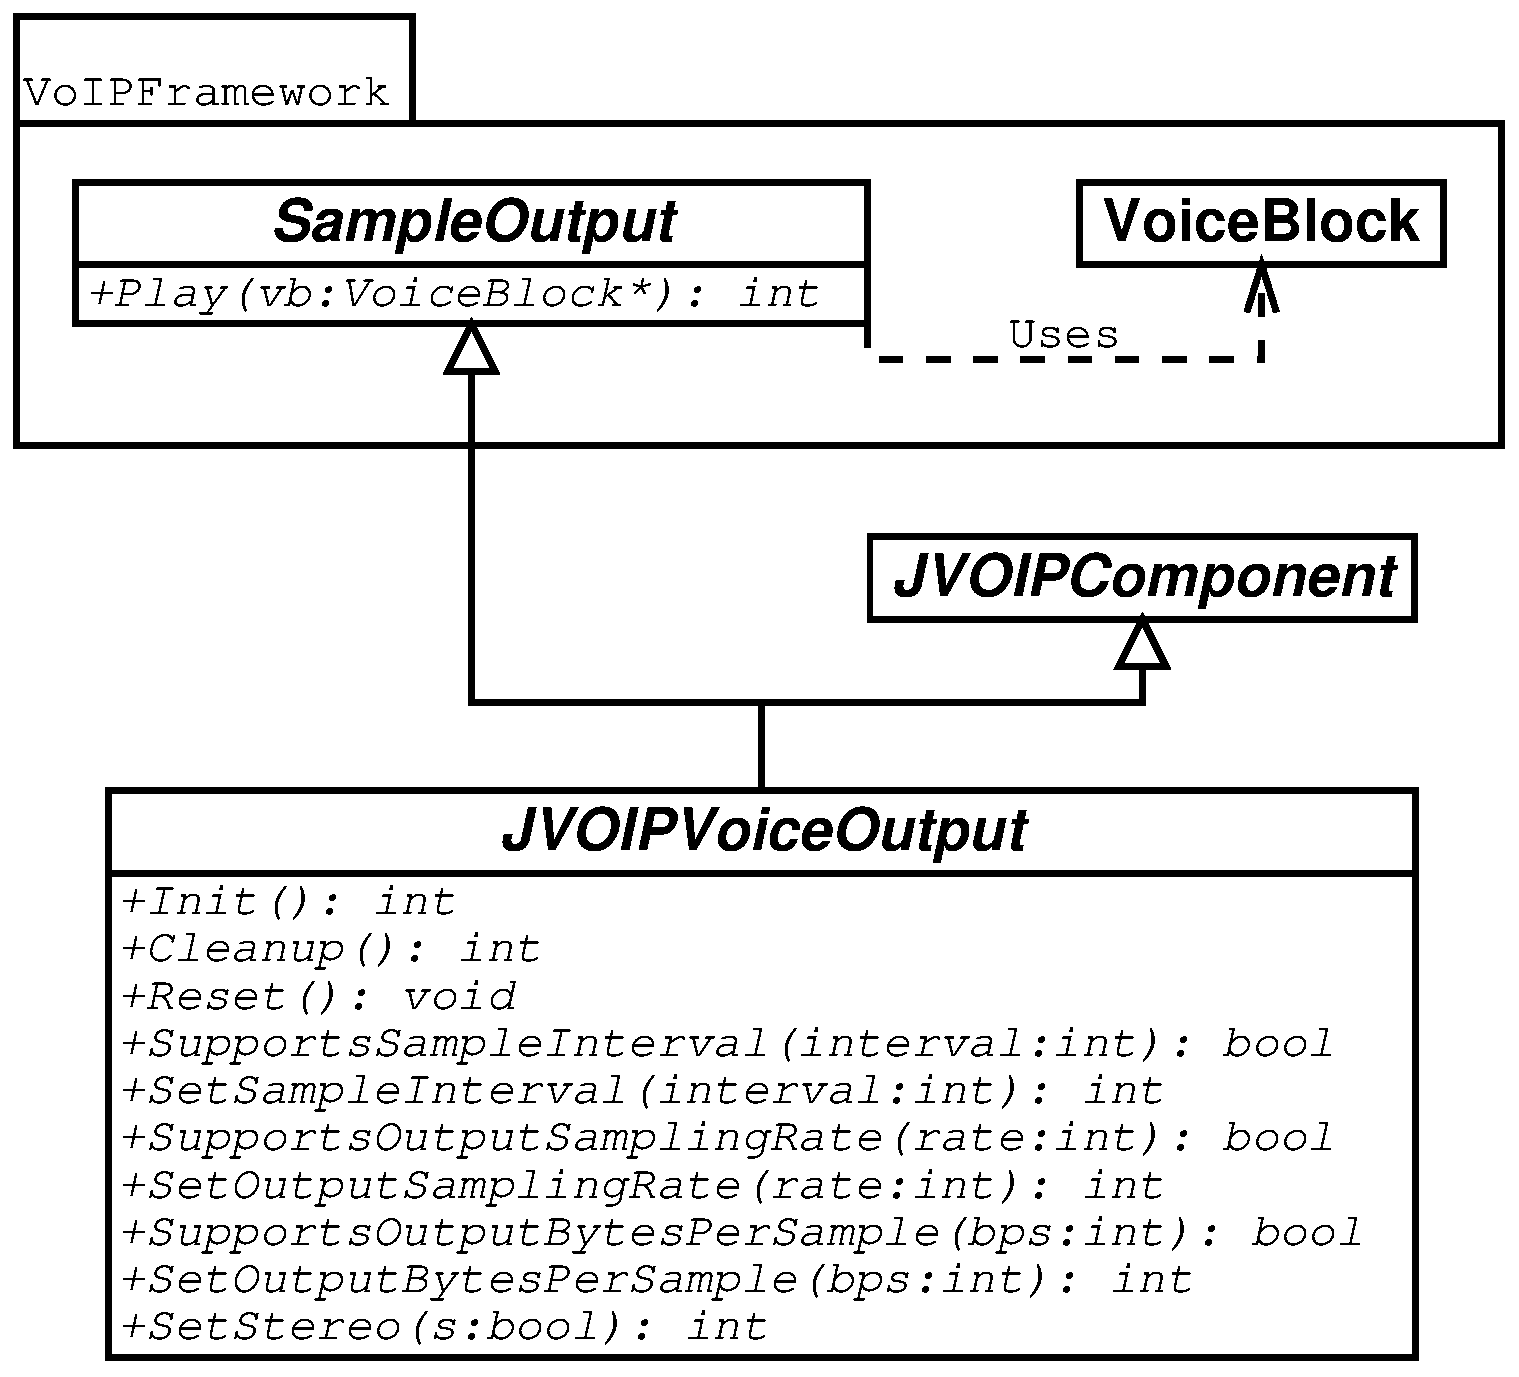
\includegraphics[width=0.8\linewidth]{images/manual/chapter2/class-jvoipvoiceoutput.eps}
				\caption{JVOIPVoiceOutput}
				\label{class-jvoipvoiceoutput}
			\end{figure}
			
			The class simply inherits from the {\tt SampleOutput} class in the
			{\tt VoIPFramework} namespace, so it can be used in the {\tt Step}
			routine from section \ref{text-voipframework-voipprocedure}.
			
			It's {\tt Init} function is more complicated than is shown in the
			figure. Here's its true form:
			\begin{center}
				{\tt
				\begin{tabular}{rl}
					int Init (&int sampinterval, int outputsamprate,\\
					&int outputbytespersample, bool stereo,\\
					&const JVOIPComponentParams *componentparams )\\
				\end{tabular}
				}
			\end{center}
			
			\subsubsection{JVOIPLocalisation \& JVOIPSessionLocalisation}
			
			If you want to implement a localisation scheme, you can do this by
			deriving a class from {\tt JVOIPLocalisation}. As is shown in figure
			\ref{class-jvoiplocalisation}, this class is derived from both
			{\tt Location3D} and {\tt Transform3D} of the {\tt VoIPFramework}
			namespace.
			\begin{figure}
				\center
				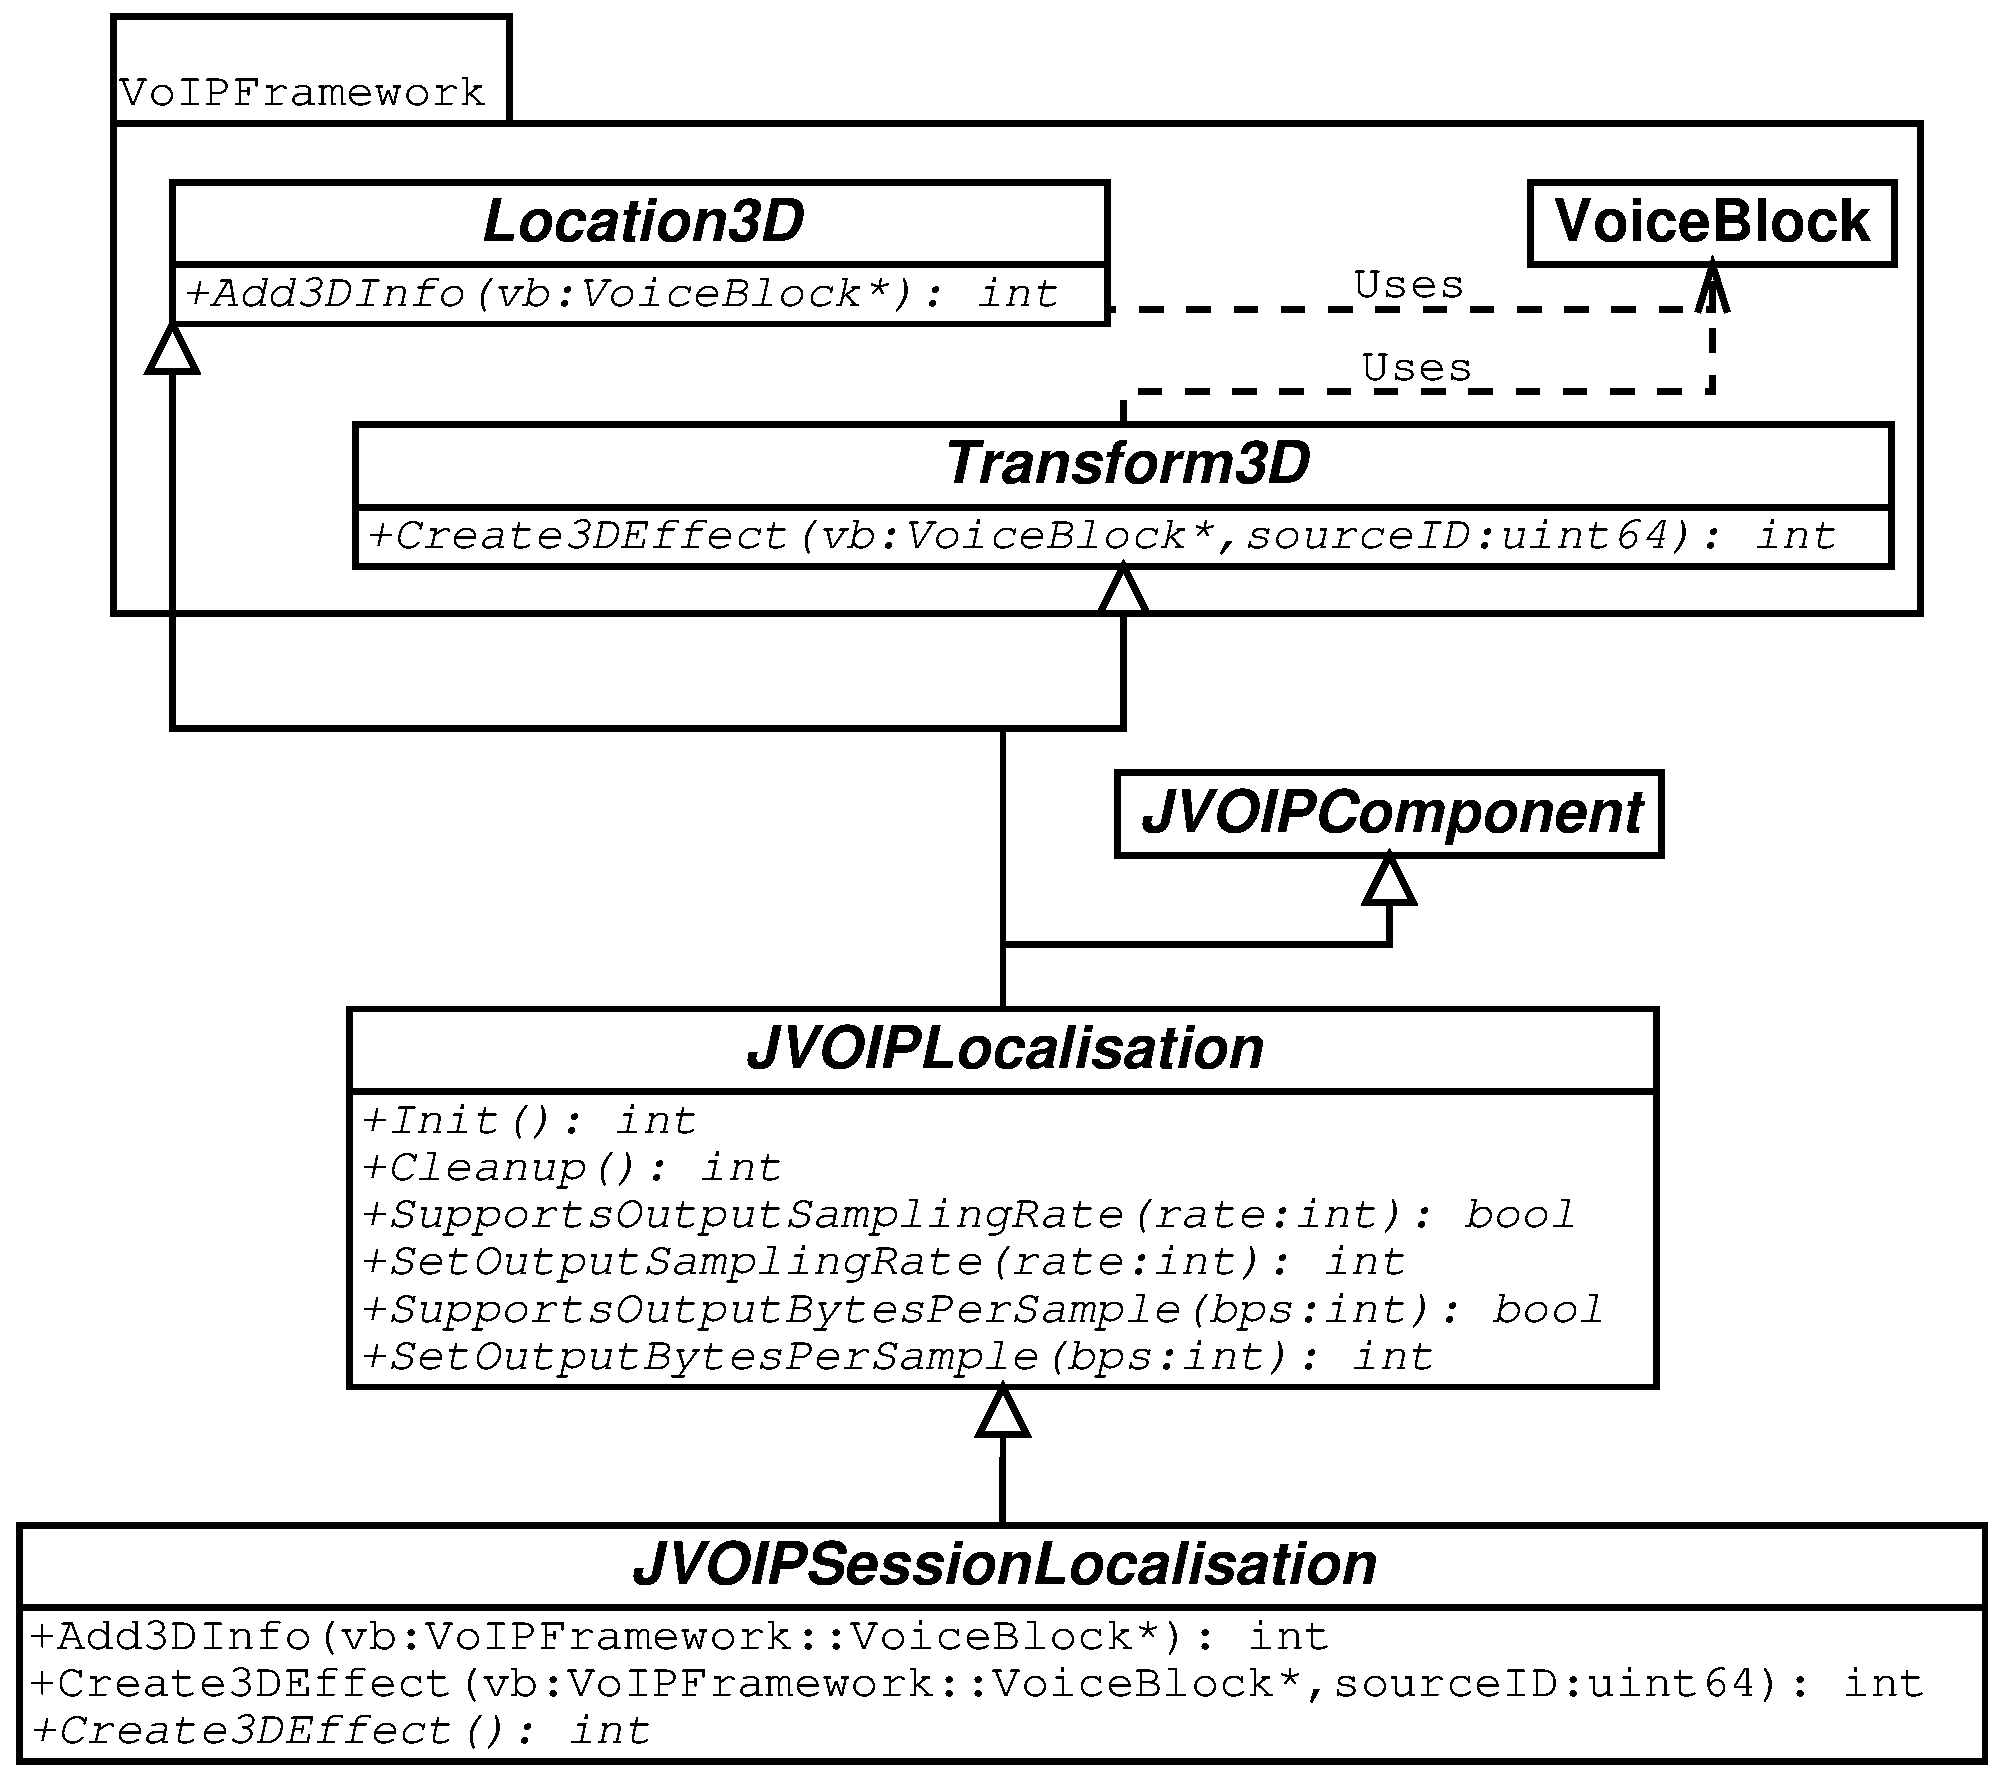
\includegraphics[width=\linewidth]{images/manual/chapter2/class-jvoiplocalisation.eps}
				\caption{JVOIPLocalisation \& JVOIPSessionLocalisation}
				\label{class-jvoiplocalisation}
			\end{figure}
			
			Again, the {\tt Init} function is not displayed correctly in the figure.
			The real function looks like this:
			\begin{center}
				{\tt
				\begin{tabular}{rl}
					int Init (&int outputsamprate, int outputbytespersample,\\
					&const JVOIPComponentParams *componentparams )\\
				\end{tabular}
				}
			\end{center}
			
			Instead of using the {\tt JVOIPLocalisation} class, you can also derive
			your class from {\tt JVOIPSessionLocalisation}. In this case, the
			{\tt Add3DInfo} and {\tt Create\-3D\-Effect\-(voice\-block, source\-ID)} methods are
			already implemented.
			
			The {\tt Add3DInfo} function will call the {\tt JVOIPSession} member function
			{\tt Encode\-Own\-Position} to store the 3D info in the {\tt VoiceBlock} instance.
			The {\tt Create\-3D\-Effect\-(voice\-block, source\-ID)} function will decode the positional
			information using the {\tt JVOIP\-Session} member function {\tt DecodePositionalInfo}.
			It will also make a call to the {\tt JVOIP\-Session} member {\tt RetrieveOwnPosition}
			and with all this information it will call a new {\tt Create\-3D\-Effect} function,
			which is also shown in the figure.
			
			The real syntax of that function was too large to fit in the image, so I'll
			present it here:
			\begin{center}
				{\tt
				\begin{tabular}{rl}
				int Create3DEffect(&double local\_x, double local\_y, double local\_z,\\
				                   &double righteardir\_x, double righteardir\_y, \\
						   &double righteardir\_z, double frontdir\_x, double frontdir\_y, \\
						   &double frontdir\_z, double updir\_x, double updir\_y, \\
						   &double updir\_z, double remote\_x, double remote\_y,\\
						   &double remote\_z, VoIPFramework::VoiceBlock *vb,\\
			                           &uint64 sourceID )\\
				\end{tabular}
				}
			\end{center}
			
			\subsubsection{JVOIPCompressionModule}
			
			Compression algorithms can be implemented using classes derived from
			{\tt JVOIP\-Compression\-Module}, shown in figure \ref{class-jvoipcompressionmodule}.
			As you can see, this class is {\em not} derived from classes of the
			VoIP framework. How can such a class then be used in the {\tt Step} procedure
			from section \ref{text-voipframework-voipprocedure}?
			\begin{figure}
				\center
				\includegraphics[width=\linewidth]{images/manual/chapter2/class-jvoipcompressionmodule.eps}
				\caption{JVOIPCompressionModule}
				\label{class-jvoipcompressionmodule}
			\end{figure}
			
			To answer this, first consider the following situation: you are having
			a VoIP call with a friend of yours and neither one of you is using
			compression. At some point, for whatever reason, you want to start using
			compression, lets say DPCM. Your friend, however, still wants to use
			uncompressed signals.
			
			If only one compression scheme can be used at a time, there would be major
			problems in the situation above. The DPCM decompressor would start trying
			to decompress the signals from your friend, but these signals were already
			uncompressed! Similarly, your friend would start to hear very strange noises
			since your DPCM compressed VoIP signals would be treated as normal, 
			uncompressed data.
			
			The solution to this problem is to use some kind of compression manager:
			during the entire session all implemented decompression routines will be
			available, so that when the compression scheme changes, another algorithm
			can be used. Since you can only use one compression algorithm at a time,
			only one compression routine needs to be initialized at any moment.
			
			This is how things are handled within JVOIPLIB. The compression manager
			is captured in the class {\tt JVOIPCompression} and this class will use
			the available compression modules (derived from {\tt JVOIP\-Compression\-Module})
			as needed. This situation is illustrated in figure \ref{class-jvoipcompression}
			\begin{figure}
				\center
				\includegraphics[width=\linewidth]{images/manual/chapter2/class-jvoipcompression.eps}
				\caption{JVOIPCompression}
				\label{class-jvoipcompression}
			\end{figure}
			
			If you take a look at figure \ref{class-jvoipcompressionmodule} again,
			you will see that each compression module will have a member function
			called {\tt InitDecompressor}. Upon initialization, the {\tt JVOIP\-Com\-pres\-sion}
			instance will initialize all available decompression algorithms by
			calling each module's {\tt InitDecompressor} function.
			
			The compression manager will also initialize the active compression
			routine by calling the {\tt InitCompressor} function of the appropriate
			compression module. This function is not displayed in its true form;
			actually it looks like this:
			\begin{center}
				{\tt
				\begin{tabular}{rl}
				int InitCompressor(&int sampinterval, int inputsamprate,\\
				&int inputbytespersample,\\
				&const JVOIPComponentParams *componentparams )
				\end{tabular}
				}
			\end{center}
			
			\subsubsection{JVOIPMixer}
			
			The mixer component is derived from {\tt VoiceMixer} in the {\tt VoIPFramework}
			namespace, as is illustrated in figure \ref{class-jvoipmixer}.
			\begin{figure}
				\center
				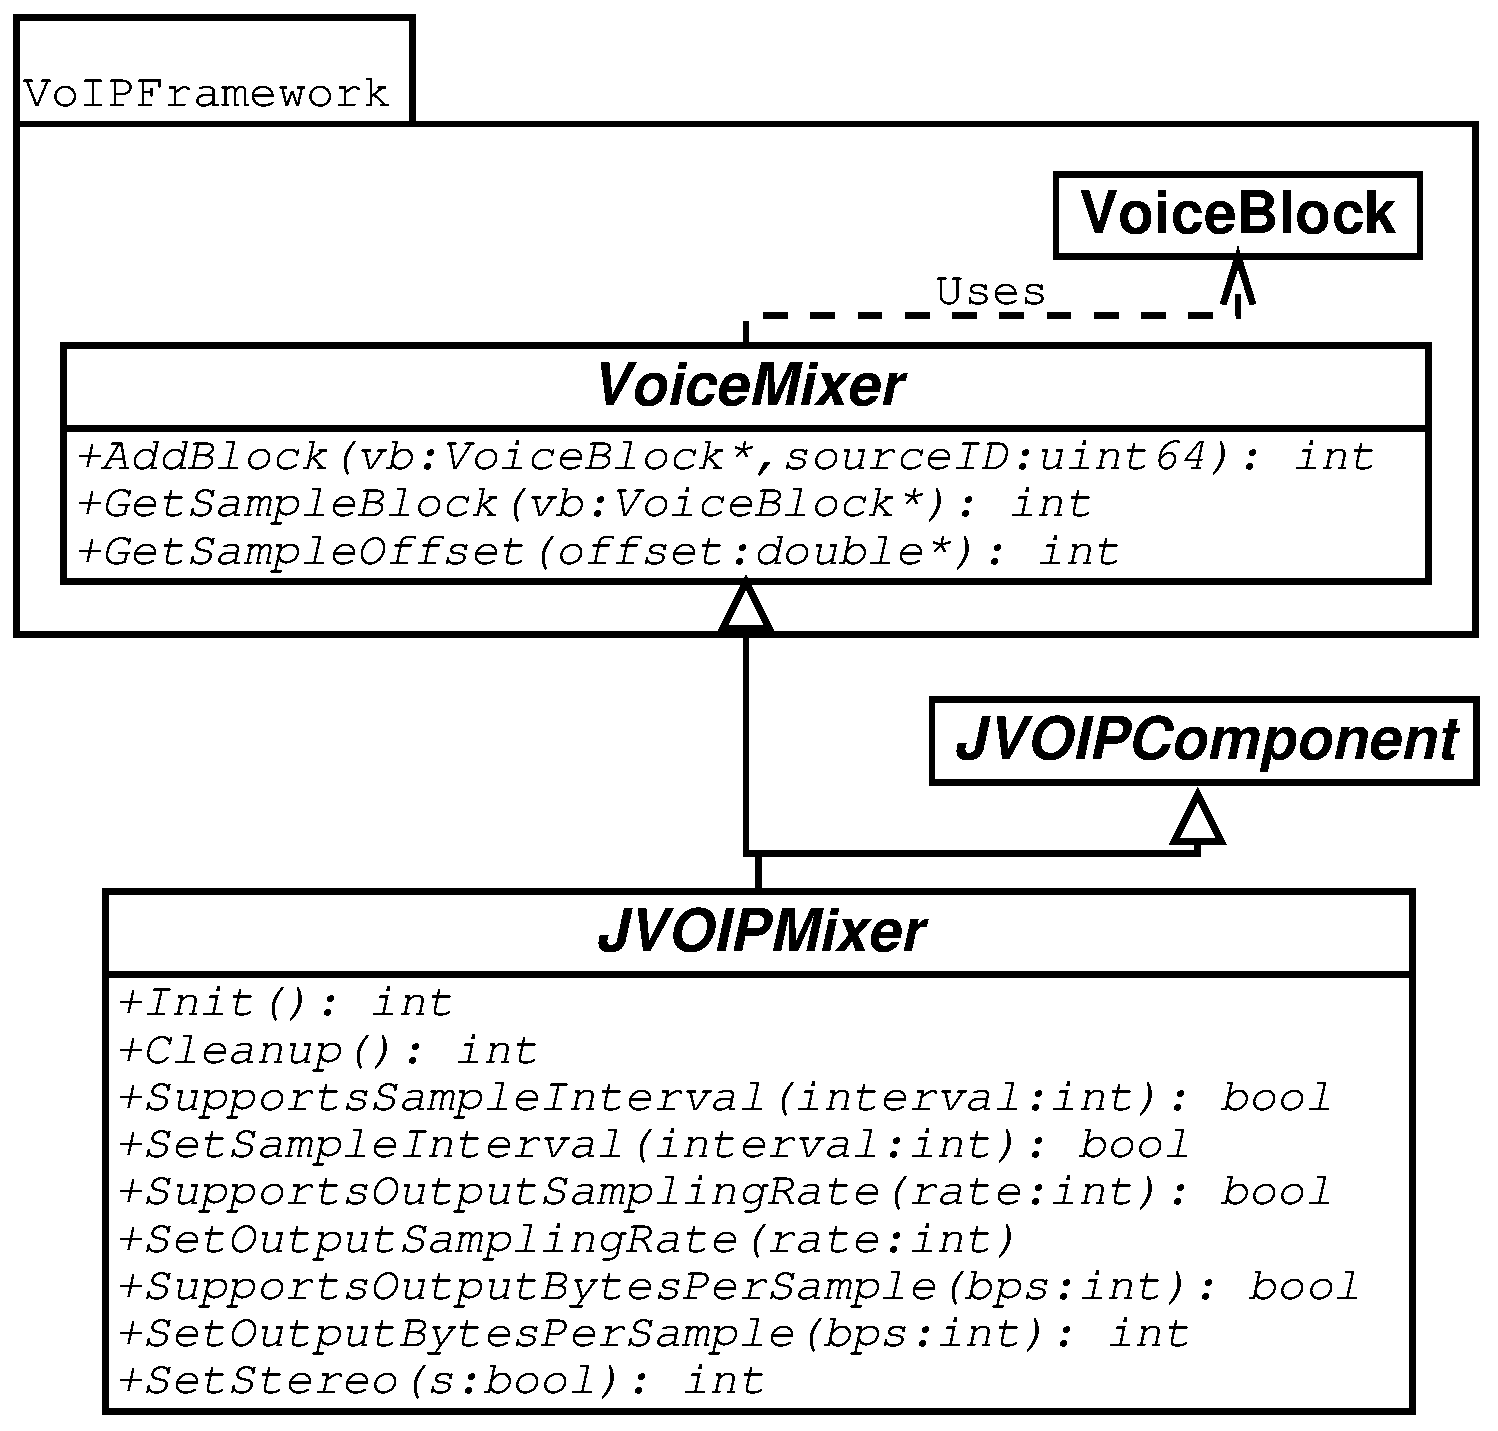
\includegraphics[width=0.8\linewidth]{images/manual/chapter2/class-jvoipmixer.eps}
				\caption{JVOIPMixer}
				\label{class-jvoipmixer}
			\end{figure}
			
			Again, the {\tt Init} function is more complex than it is in the figure. The
			function declaration is as follows:
			\begin{center}
				{\tt
				\begin{tabular}{rl}
				int Init(&int sampinterval, int outputsamprate,\\
				&int outputbytespersample, bool stereo,\\
				&const JVOIPComponentParams *componentparams )\\
				\end{tabular}
				}
			\end{center}
			
			\subsubsection{JVOIPTransmission}
			
			The last component is represented by the class {\tt JVOIPTransmission}. This
			class is derived from {\tt VoiceTransmitter} in the {\tt VoIPFramework} namespace.
			This situation is shown in figure \ref{class-jvoiptransmission}.
			\begin{figure}
				\center
				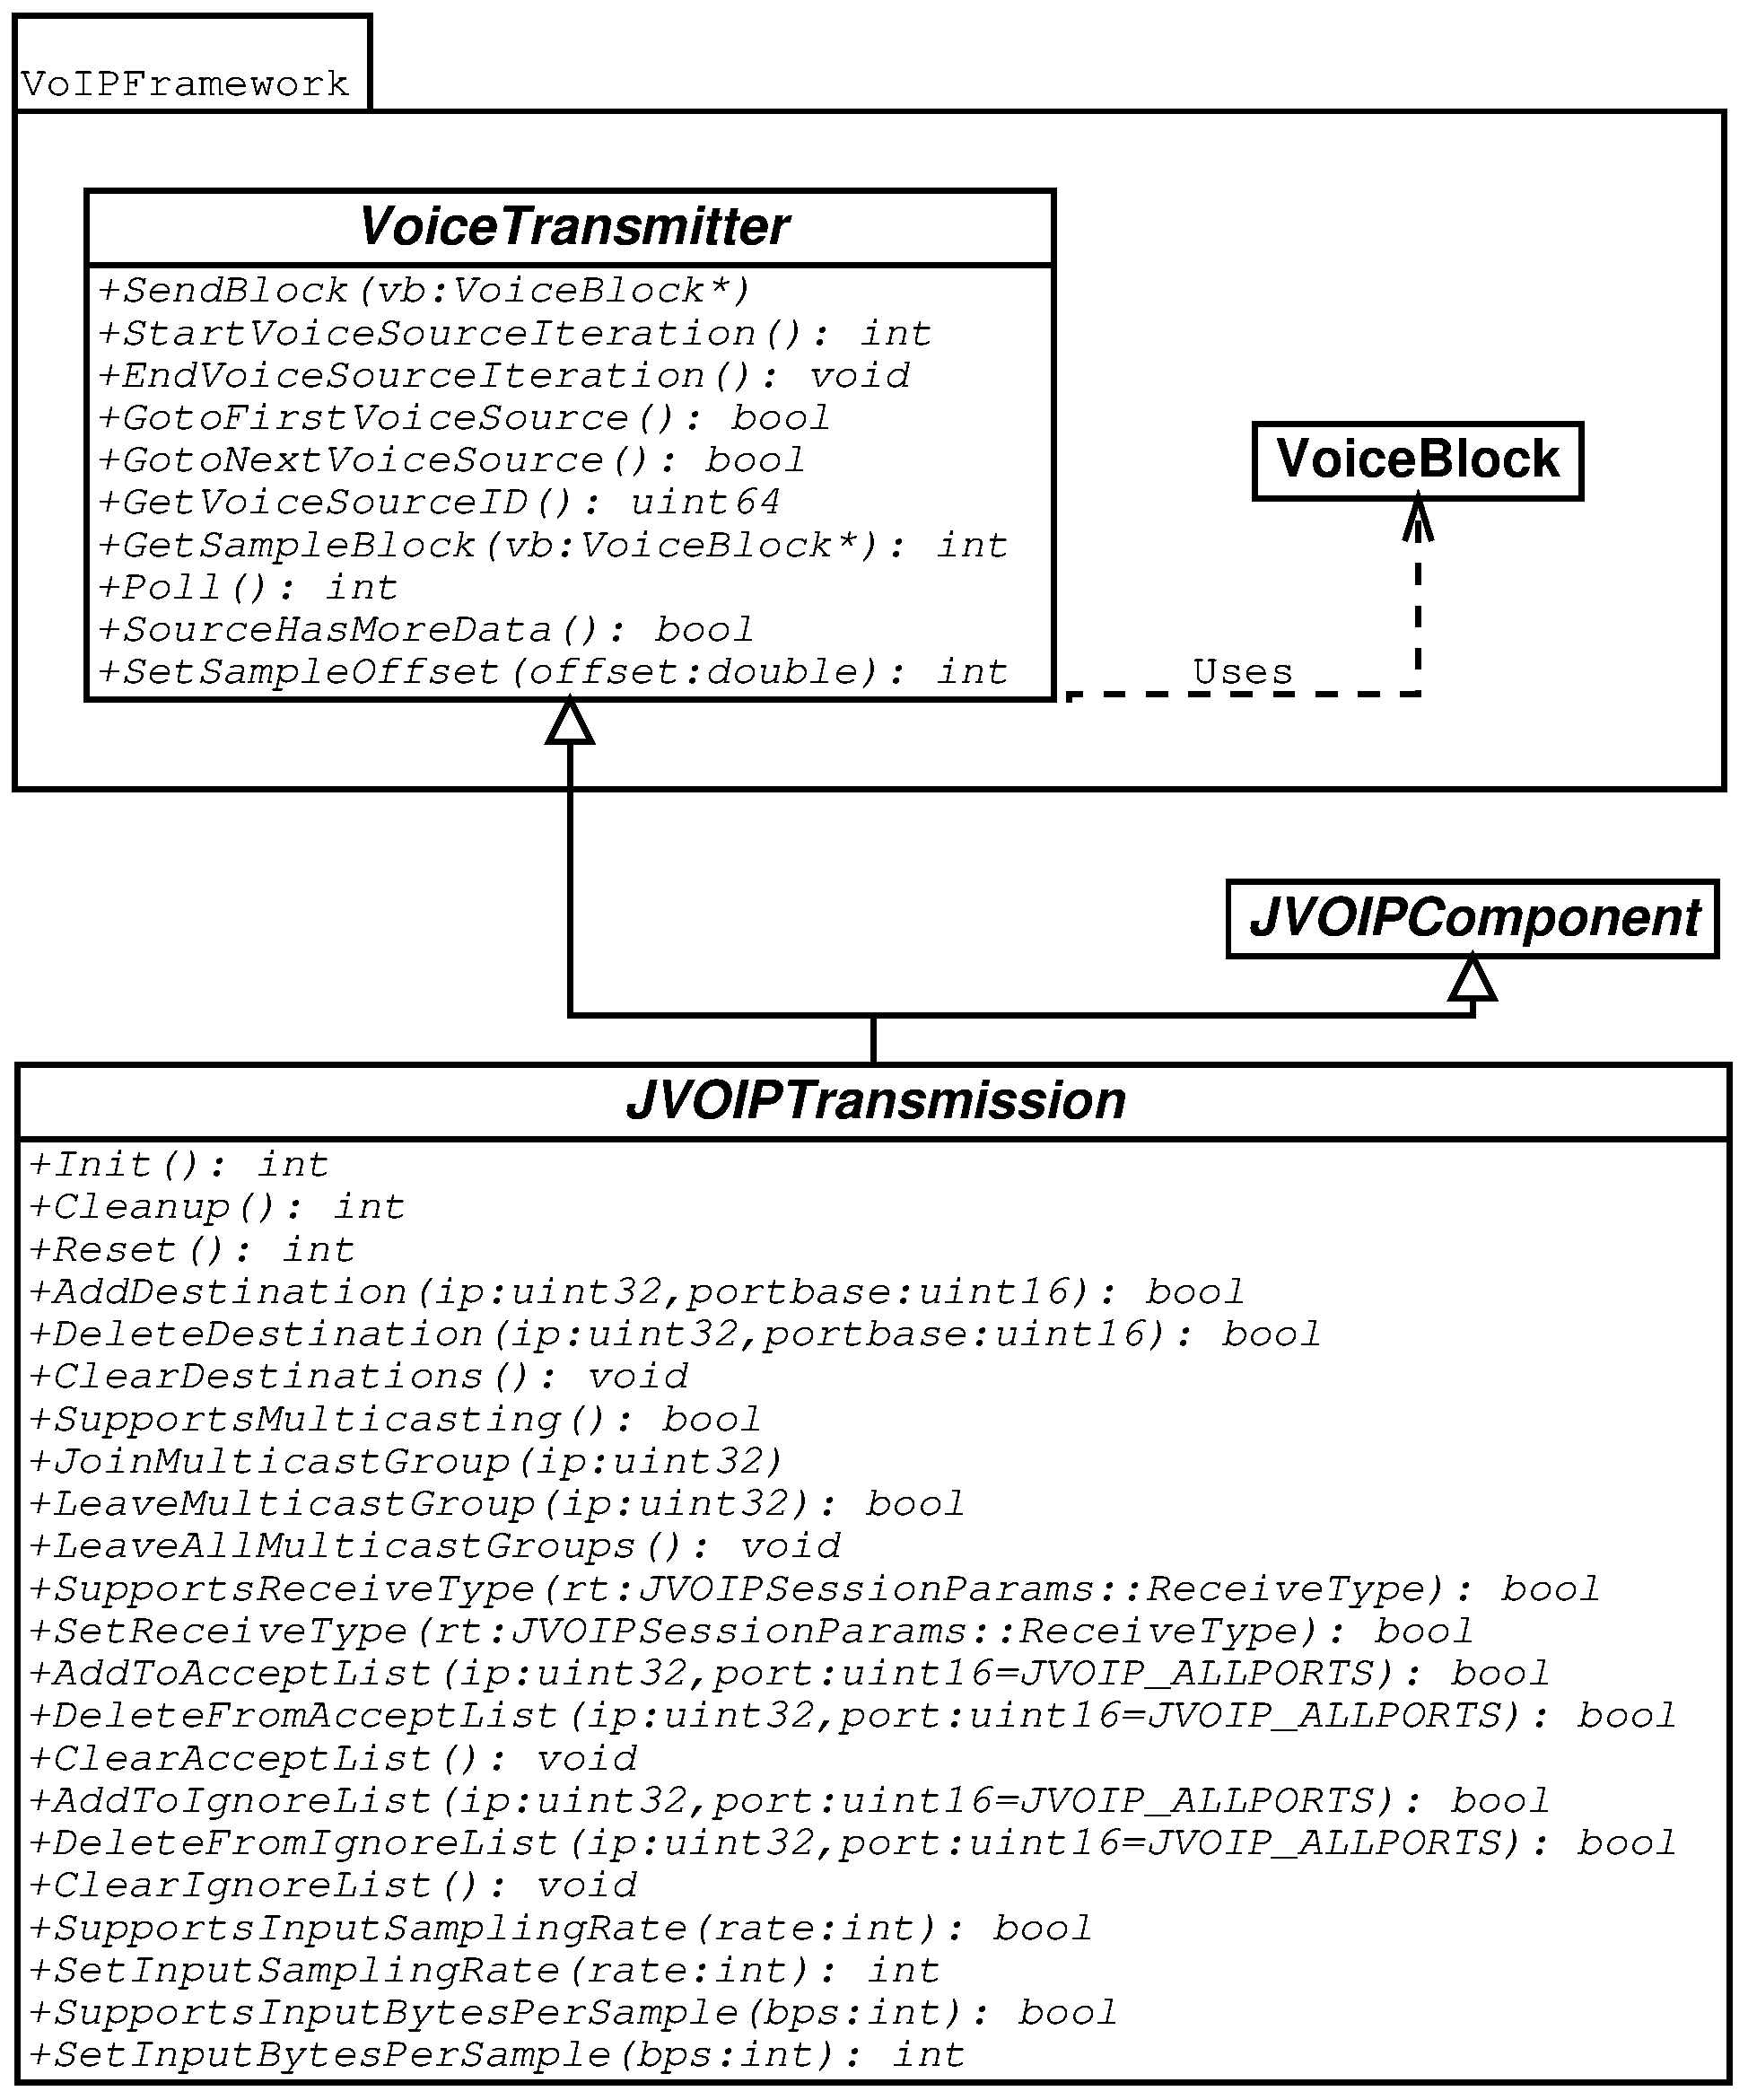
\includegraphics[width=\linewidth]{images/manual/chapter2/class-jvoiptransmission.eps}
				\caption{JVOIPTransmission}
				\label{class-jvoiptransmission}
			\end{figure}
			
			In section \ref{text-voipframework-voipprocedure}, the main VoIP routine
			was explained. At a certain point in the {\tt Step} routine, there was
			this piece of pseudo code:
			\begin{lstlisting}[frame=tb]{}
		for (each voice source with available data)
		{
			do
			{
				...
			} while (voice source has more data);
		}
			\end{lstlisting}
			
			Using the functions of the {\tt VoiceTransmitter} class, this is done
			like this:
			\begin{lstlisting}[frame=tb]{}
		if (voicetransmitter->GotoFirstVoiceSource())
		{
			do
			{
				do
				{
					...
				} while (voicetransmitter->SourceHasMoreData());
			} while (voicetransmitter->GotoNextVoiceSource());
		}
			\end{lstlisting}
			
			The syntax of the {\tt Init} function of the {\tt JVOIPTransmission} class is
			not accurate in the figure. Actually, it's this:
			\begin{center}
				{\tt
				\begin{tabular}{rl}
				int Init(&int sampinterval, int inputsamprate, int inputbytespersample,\\
				&const JVOIPComponentParams *componentparams )\\
				\end{tabular}
				}
			\end{center}
